\section{Planning}
\SectionPage

\begin{frame}
  \frametitle{Features}
  \begin{itemize}
    \item Easy to extend (with modules)
      \pause
      \begin{itemize}
        \item Low bar to create a module
          \pause
        \item Easy to reason about how modules work together
          \pause
      \end{itemize}
    \item Proof-of-concept modules should extend the application to include
      these features:
      \pause
      \begin{itemize}
        \item Can open, edit, delete files
          \pause
        \item Has LSP support
          \pause
        \item Can compile and execute a program
      \end{itemize}
  \end{itemize}
\end{frame}

\begin{frame}
  \frametitle{Goals}
  % TODO: Should probably make these points more concrete
  \begin{itemize}
    \item Should be better than the current IDE
      \pause
      \begin{itemize}
        \item Easy installation
      \end{itemize}
      \pause
    \item Easy for the next \sout{sucker} developer to change core functionality
      \pause
      \begin{itemize}
        \item Good CI-CD
        \pause
        \item Good documentation
        \pause
      \end{itemize}
    \item Have a good module developer experience
      \begin{itemize}
          \pause
        \item Language Agnostic Module Architecture
          \pause
        \item Good debugging tools
      \end{itemize}
  \end{itemize}
\end{frame}

\begin{frame}
  \frametitle{What Is A Module?}
  \begin{itemize}
    \item Third Party Code to be executed/interpreted
      \pause
      \begin{itemize}
        \item Tailor made Scripting Language
          \pause
          \begin{itemize}
            \item Vim Script (Vim)
              \pause
          \end{itemize}
        \item An already existing programming language
        \pause
          \begin{itemize}
            \item Lua (NeoVim)
            \pause
            \item JavaScript (VS Code)
            \pause
            \item Java/Kotlin/Clojure (Eclipse/IntelliJ)
          \end{itemize}
      \end{itemize}
  \end{itemize}
\end{frame}

\begin{frame}
  \frametitle{Granularity}
  \begin{itemize}
    \item How \textit{big} is a module?
      \pause
      \begin{itemize}
        \item Could create a module which enables some feature $A$
          \pause
          \begin{itemize}
            \item Not very granular
          \end{itemize}
          \pause
        \item Could create a module for each function, needed to enable feature
            $A$
          \begin{itemize}
              \pause
            \item Very granular
          \end{itemize}
        \item More granular $\implies$ more complex
        \pause
          \begin{itemize}
            \item More granular $\implies$ less repetition
           \pause
          \end{itemize}
        \item Less granular $\implies$ less complex
        \pause
          \begin{itemize}
            \item Less granular $\implies$ more repetition
            \pause
          \end{itemize}
      \end{itemize}
  \end{itemize}
\end{frame}

% NOTE: Should go in depth about how a module family can be treated as a
% singular module, by a consumer
\hidelogo
\begin{frame}
  \frametitle{Module Family}
  \begin{itemize}
    \item Grouping of related modules that work together.
      \pause
    \item Example
      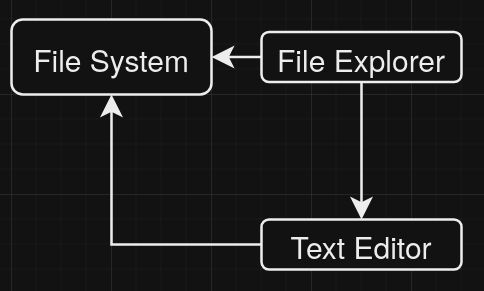
\includegraphics[width=0.9\textwidth]{./pics/ide-family.png}
  \end{itemize}
\end{frame}

\showlogo
\section{Modeling a Module}
\SectionPage

\begin{frame}
  \frametitle{How To model A Module?}
  \begin{itemize}
    \item A module needs to:
      \pause
      \begin{itemize}
        \item Initialize some state
          \pause
        \item Update the state based on events
          \pause
        \item Change the view based on the state
      \end{itemize}
      \pause
    \item Module architecture is inspired by Elm and MVC
      \pause
    \item A module should be \textit{pure}
  \end{itemize}
\end{frame}

\begin{frame}
  \frametitle{Module V.1}
  \begin{itemize}
    \item First plan
      \pause
      \begin{enumerate}
        \item Create an IDE
          \pause
        \item Extend the IDE, to allow for a module architecture
          \pause
        \item Modules call the application using some DSL
          \pause
      \end{enumerate}
    \item Pros
      \pause
      \begin{itemize}
        \item \textit{Easy} to implement
          \pause
        \item Get a good understanding of what features might be needed
          \pause
        \item And therefore how the IDE module API should look like
      \end{itemize}
    \item Cons
      \pause
      \begin{itemize}
        \item Not really modular
          \pause
        \item Will be subpar compared to existing software
          \pause
        \item Impossible to know all use cases for the API
      \end{itemize}
  \end{itemize}
\end{frame}

\begin{frame}
  \frametitle{Module V.1 - Final}
  \begin{itemize}
    \item Second plan
      \pause
      \begin{enumerate}
          % TODO: Add footnote
        \item Everything* is a module
      \end{enumerate}
      \pause
      \begin{itemize}
        \item A module exposes three functions, that are invoked by the core
          \pause
          \begin{itemize}
            \item Init - Returns a set of fields, which are added to the core state
              \pause
            \item Update - Returns a set of fields which are updated
              \pause
            \item View - Returns a set which represents HTML, which is rendered by
              the core
          \end{itemize}
          \pause
        \item Easy to keep modules pure
          \pause
        \item Optimization is possible due to the pureness of modules
          \pause
        \item Easy to reason about module cooperation
      \end{itemize}
  \end{itemize}
\end{frame}

\hidelogo
\begin{frame}
  \frametitle{Example}
  \begin{figure}
    \centering
    \begin{minted}{haskell}
-- Manifest :: Map
init :: Map
init :: [("counter", ValInt 0)]

update :: Msg -> Map -> Map
update (PluginMsg "counter") model =
  case lookup "counter" model of
    Just (ValInt i) -> insert "counter" (ValInt (i + 1)) model
    Nothing -> insert "counter" (ValInt 0) model

view :: Map -> Html
view model = Div [] [Text "Hello, World!"
  , Btn [OnClick (PluginMsg "counter")] []
  , Text (putStrLn (lookupOrDefault "counter" model))
\end{minted}



    \caption{Example Module Architecture}
    \label{fig:moduleArchitecture}
  \end{figure}
\end{frame}

\showlogo
\begin{frame}
  \frametitle{Example Types for State}
    \begin{center}
      \lstinputlisting
      [ language=Haskell
      , caption={State representation in Haskell}
      , label=lst:pluginState
      ]{./code/plugin-types-state.hs}
    \end{center}
\end{frame}

\begin{frame}
  \frametitle{Example Types for Msg and HTML}
    \begin{center}
      \lstinputlisting
      [ language=Haskell
      , caption={Example Types for Msg and HTML}
      , label=lst:pluginTypes
      ]{./code/plugin-types.hs}
    \end{center}
\end{frame}

\section{Implementation}
\SectionPage

\begin{frame}
  \frametitle{Tech \sout{Heap} Stack}
  \begin{itemize}
    \item Rust, because it is a low level system language
      \pause
      \begin{itemize}
        \item Compiler knows when a value is unused
          \pause
        \item Automatically \textit{dropped}
          \pause
        \item No dangling pointers/null references
      \end{itemize}
      \pause
    \item Tauri, UI components can be created using JavaScript
      \pause
    \item Splits the core application in two, loosely coupled parts
      \begin{itemize}
        \item Frontend (JavaScript)
          \pause
        \item Backend (Rust)
      \end{itemize}
      \pause
    \item Communication is like JSON-RPC, which, effectively, is the same as a
      client-server
      \pause
    \item Allows for modules in two different languages, with little effort.
      I hoped.
  \end{itemize}
\end{frame}

\begin{frame}
  \frametitle{Blasingly Fast Memory Leakage}
  \begin{itemize}
    \item The Rust ABI is not protected by their semver notation
      \pause
    \item This means that even a patch to the Rust compiler can break a
      Rust Module
      \pause
    \item Can be fixed by using a Rust Library: \textit{abi\_stable}
      \pause
    \item Had to use `ManuallyDrop` for more complex types, which disables
      the automatic drop
      \pause
    \item Fixed by having Rust modules only reference the state, meaning
      after update and view, the module can be safely dropped
  \end{itemize}
\end{frame}

\begin{frame}
  \frametitle{I Need Super Computer Time For My Featureless App}
  \begin{itemize}
      \pause
    \item JavaScript is more \textit{unsafe} than Rust, due of a lack of typing
      \pause
    \item Need to decode the output from the modules, and catch any exceptions
      \pause
    \item When implementing the init to update to view - cycle, I tested with
      a \textit{basic} module, which should only display "Hello, World!"
      \begin{itemize}
          \pause
        \item The module initialized the state
          \pause
        \item It rendered the view
          \pause
        \item Somehow triggered an update
          \pause
        \item Which triggered a re-render
          \pause
        \item Which triggered an update
          \pause
        \item Which triggered a re-render
          \pause
        \item \dots
      \end{itemize}
  \end{itemize}
\end{frame}

\begin{frame}
  \frametitle{I Need Super Computer Time For My Featureless App}
  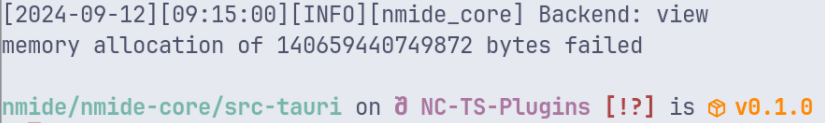
\includegraphics[width=0.9\textwidth]{./pics/memory-allocation-zoomed.png}
\end{frame}

\begin{frame}
  \begin{itemize}
    \item State is append-only
      \pause
    \item State can only grow
      \pause
    \item Not really modular
      \pause
    \item No Module-to-Module communication/invocation
    \item No stable ABI; complicates module language agnosticism
    \item Redundant updates and re-renderings
    \item Complex resolution and detection of state collisions
  \end{itemize}
\end{frame}

\showlogo
\begin{frame}
  \frametitle{Module V.1 - Final.Final}
  \begin{itemize}
    \item Third, and hopefully the final plan
      \pause
      \begin{enumerate}
        \item Everything* is a module
          \pause
        \item Modules can \textit{invoke} modules
          \pause
      \end{enumerate}
      \begin{itemize}
        \item Init - Returns a set of modifications
      \end{itemize}
      \pause
    \item Pros
      \pause
      \begin{itemize}
        \item Modular
          \pause
        \item Modules can \textit{invoke} other modules
      \end{itemize}
      \pause
    \item Cons
      \begin{itemize}
          \pause
        \item Complex to implement
      \end{itemize}
  \end{itemize}
\end{frame}

\begin{frame}
  \frametitle{Example}
  \begin{center}
    \lstinputlisting
    [ language=Haskell
    , caption={Example Plugin}
    , label=lst:moduleExample
    ]{./code/module-example.hs}
  \end{center}
\end{frame}


\begin{frame}
  \frametitle{Example Event}
  \begin{center}
    \lstinputlisting
    [ language=Haskell
    , caption={Example Plugin}
    , label=lst:moduleEvent
    ]{./code/module-example-event.hs}
  \end{center}
\end{frame}


\begin{frame}
  \frametitle{Example Counter}
  \begin{center}
    \lstinputlisting
    [ language=Haskell
    , caption={Example Plugin}
    , label=lst:moduleCounter
    ]{./code/module-example-counter.hs}
  \end{center}
\end{frame}


\begin{frame}
  \frametitle{Example Counter Handler}
  \begin{center}
    \lstinputlisting
    [ language=Haskell
    , caption={Example Plugin}
    , label=lst:moduleCounterHandler
    ]{./code/module-example-counter-handler.hs}
  \end{center}
\end{frame}
